\section{Long-Only Q1 Performance Heatmap}
\label{app:q1-heatmap}

Figure~\ref{fig:q1-heatmap} shows the top-quintile (Q1) long-only performance heatmap, complementing the long--short summary in Table~\ref{tab:longshort}.
It is useful for separating models that simply ride the broad market in Q1 from models whose bottom-quintile avoidance creates a stronger spread.

\begin{figure}[H]
  \centering
  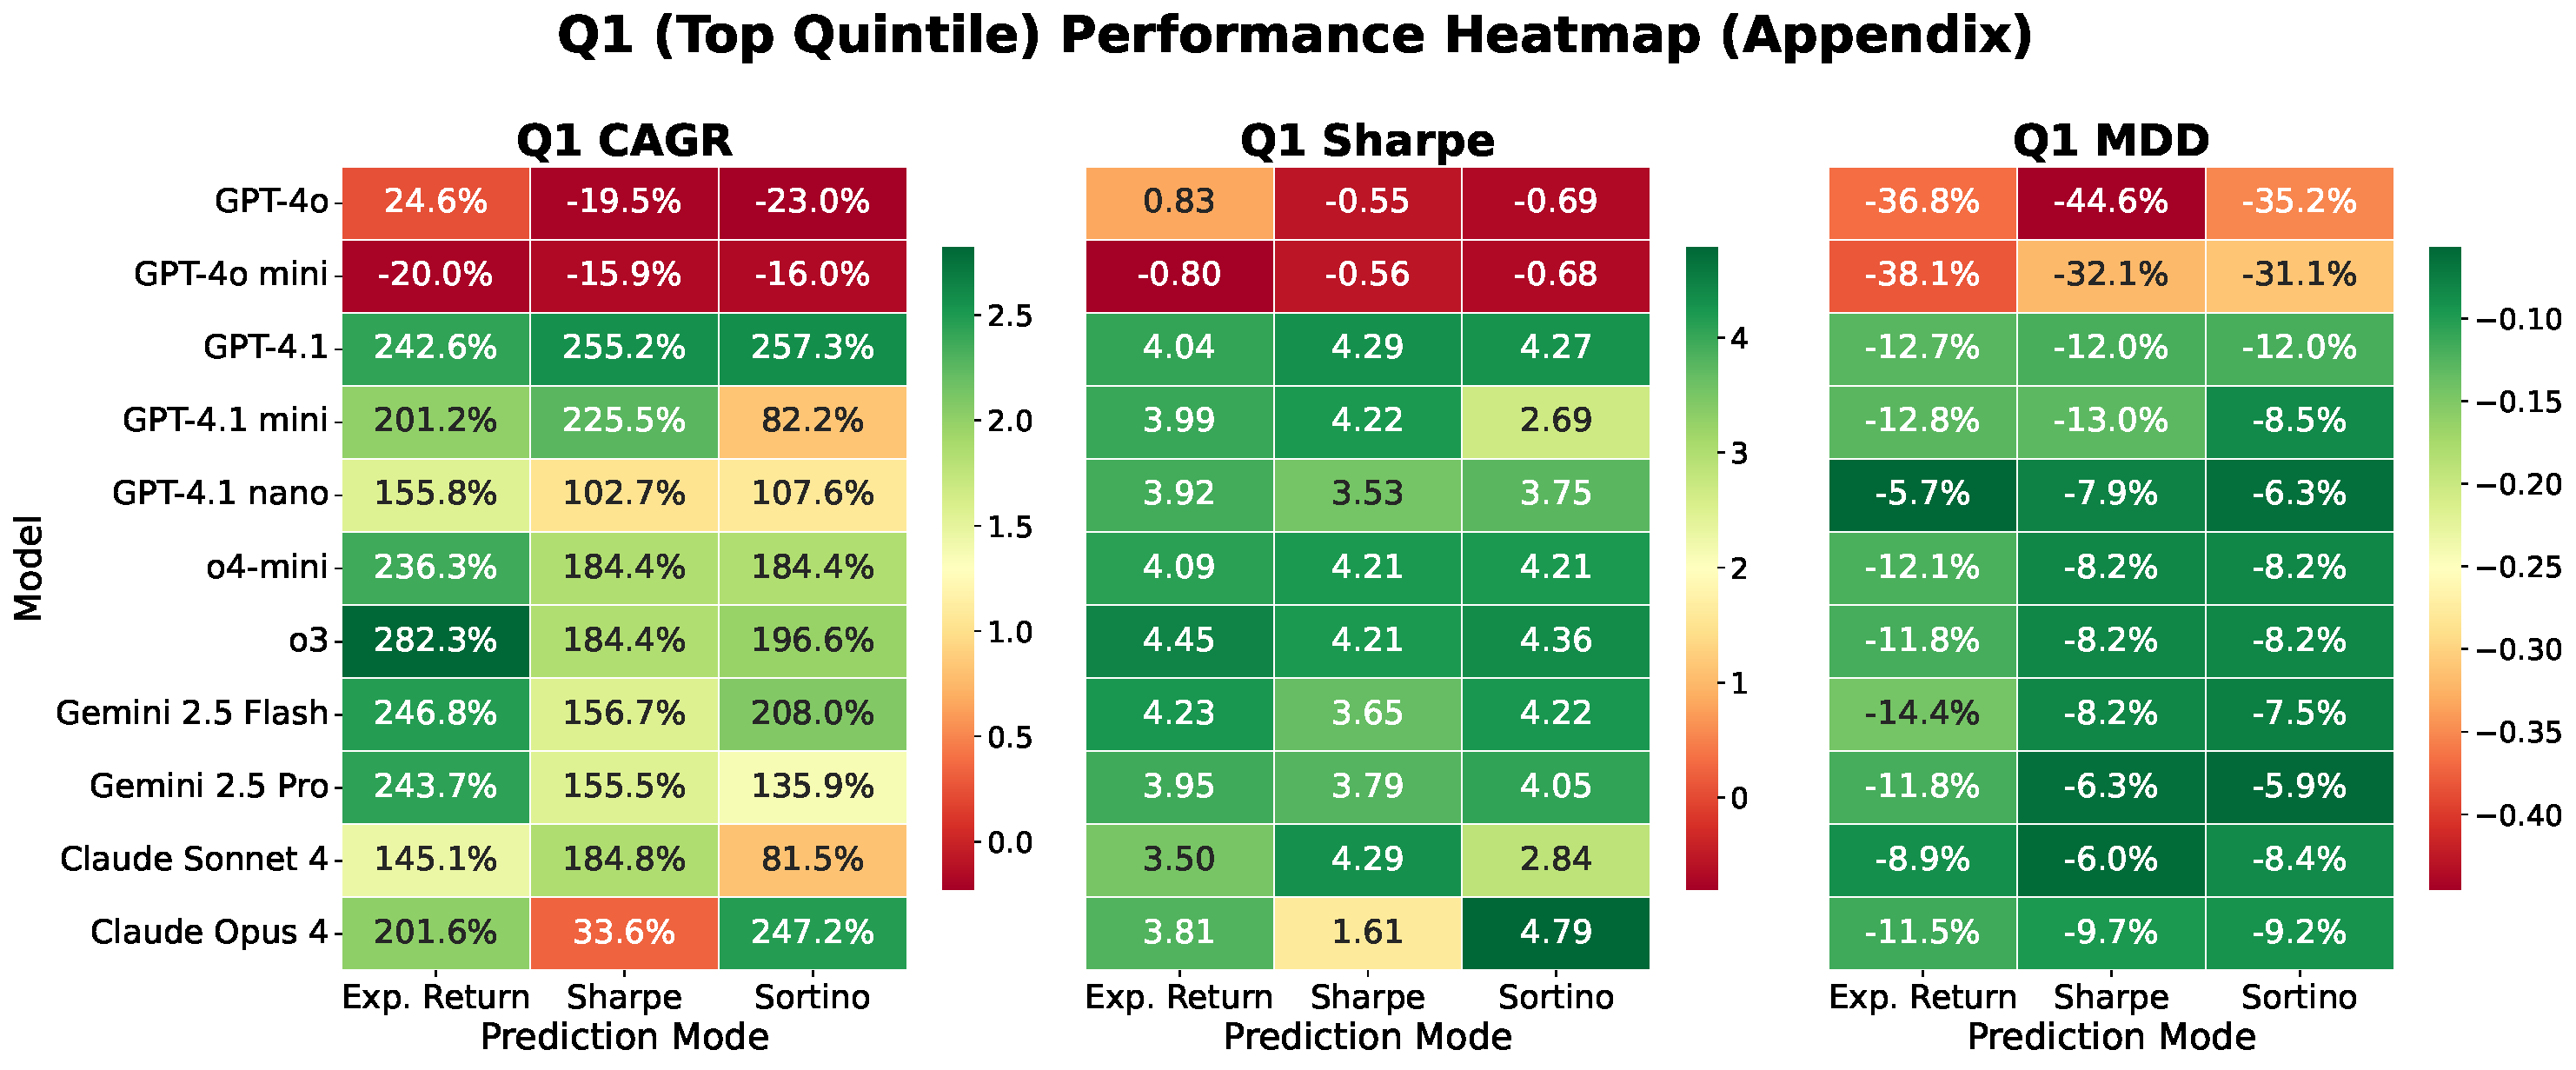
\includegraphics[width=\textwidth]{figures/fig7_q1_performance_heatmap.pdf}
  \caption{Performance heatmap of Q1 long-only portfolios by model and prediction mode. Green indicates stronger values; MDD is inverted.}
  \Description{Heatmap of long-only top-quintile CAGR, Sharpe, and maximum drawdown by model and prompt objective, with green indicating better values and red indicating worse values.}
  \label{fig:q1-heatmap}
\end{figure}

The heatmap shows that high Q1 returns are not identical to robust ranking skill.
Models can look attractive on long-only CAGR while still producing weaker market-neutral separation if their bottom quintile also benefits from the same market regime.
This is why the main benchmark reports Q1 metrics, Q1$-$Q5 spreads, and IC together.

% ──────────────────────────────────────────────────────────────
\clearpage
